\documentclass[11pt,a4paper]{report}
\usepackage[textwidth=37em,vmargin=30mm]{geometry}
\usepackage{calc,xunicode,amsmath,amssymb,paralist,enumitem,tabu,booktabs,datetime2,xeCJK,xeCJKfntef,listings}
\usepackage{tocloft,fancyhdr,tcolorbox,xcolor,graphicx,eso-pic,xltxtra,xelatexemoji}

\newcommand{\envyear}[0]{2025}
\newcommand{\envdatestr}[0]{2025-03-16}
\newcommand{\envfinaldir}[0]{webdb/2025/20250316/final}

\usepackage[hidelinks]{hyperref}
\hypersetup{
    colorlinks=false,
    pdfpagemode=FullScreen,
    pdftitle={Web Digest - \envdatestr}
}

\setlength{\cftbeforechapskip}{10pt}
\renewcommand{\cftchapfont}{\rmfamily\bfseries\large\raggedright}
\setlength{\cftbeforesecskip}{2pt}
\renewcommand{\cftsecfont}{\sffamily\small\raggedright}

\setdefaultleftmargin{2em}{2em}{1em}{1em}{1em}{1em}

\usepackage{xeCJK,xeCJKfntef}
\xeCJKsetup{PunctStyle=plain,RubberPunctSkip=false,CJKglue=\strut\hskip 0pt plus 0.1em minus 0.05em,CJKecglue=\strut\hskip 0.22em plus 0.2em}
\XeTeXlinebreaklocale "zh"
\XeTeXlinebreakskip = 0pt


\setmainfont{Brygada 1918}
\setromanfont{Brygada 1918}
\setsansfont{IBM Plex Sans}
\setmonofont{JetBrains Mono NL}
\setCJKmainfont{Noto Serif CJK SC}
\setCJKromanfont{Noto Serif CJK SC}
\setCJKsansfont{Noto Sans CJK SC}
\setCJKmonofont{Noto Sans CJK SC}

\setlength{\parindent}{0pt}
\setlength{\parskip}{8pt}
\linespread{1.15}

\lstset{
	basicstyle=\ttfamily\footnotesize,
	numbersep=5pt,
	backgroundcolor=\color{black!5},
	showspaces=false,
	showstringspaces=false,
	showtabs=false,
	tabsize=2,
	captionpos=b,
	breaklines=true,
	breakatwhitespace=true,
	breakautoindent=true,
	linewidth=\textwidth
}






\newcommand{\coverpic}[2]{
    % argv: itemurl, authorname
    Cover photo by #2~~(\href{#1}{#1})
}
\newcommand{\makeheader}[0]{
    \begin{titlepage}
        % \newgeometry{hmargin=15mm,tmargin=21mm,bmargin=12mm}
        \begin{center}
            
            \rmfamily\scshape
            \fontspec{BaskervilleF}
            \fontspec{Old Standard}
            \fontsize{59pt}{70pt}\selectfont
            WEB\hfill DIGEST
            
            \vfill
            % \vskip 30pt
            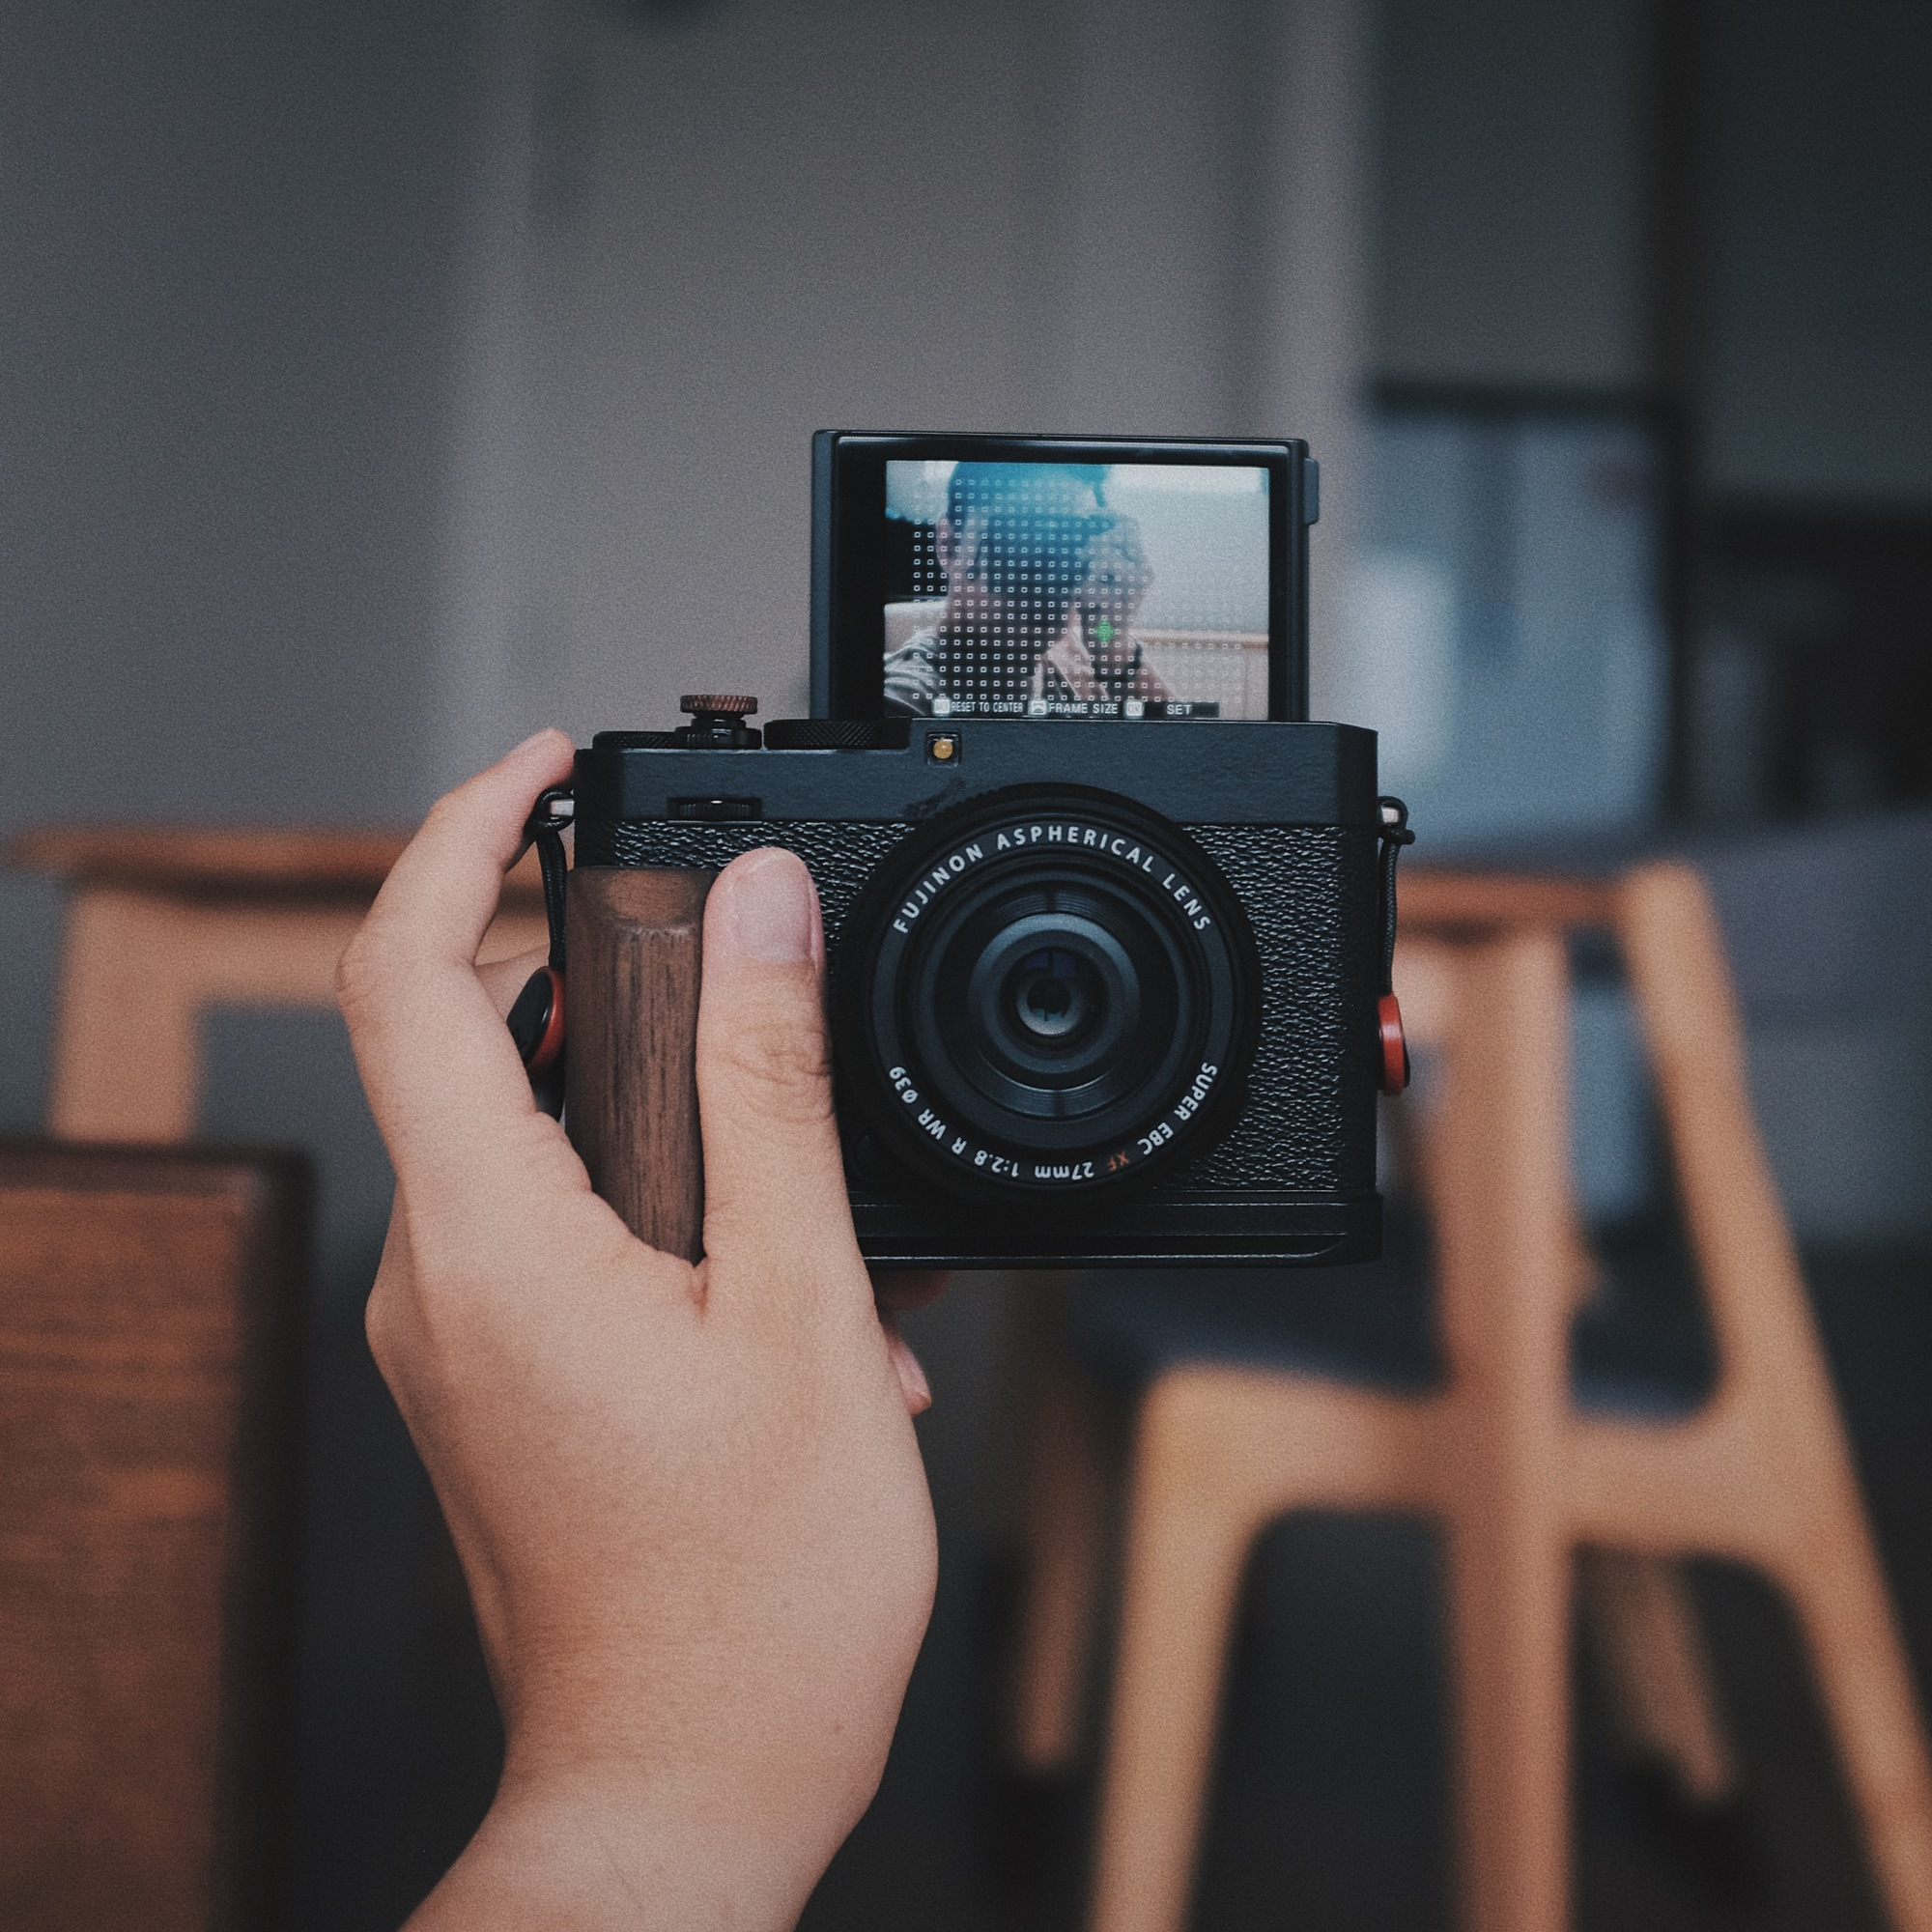
\includegraphics[width=\linewidth]{\envfinaldir/coverpic-prod.jpg}\par
            % \vskip 30pt
            \vfill

            \normalsize\rmfamily\scshape
            \copyright{} The Web Digest Project \hfill\large \envdatestr
        \end{center}
    \end{titlepage}
    % \restoregeometry
}
\newcommand{\simplehref}[1]{%
    \textcolor{blue!80!green}{\href{#1}{#1}}%
}
\renewcommand{\contentsname}{\center\Huge\sffamily\bfseries Contents\par\vskip 20pt}
\newcounter{ipartcounter}
\setcounter{ipartcounter}{0}
\newcommand{\ipart}[1]{
    % \vskip 20pt
    \clearpage
    \stepcounter{ipartcounter}
    \phantomsection
    \addcontentsline{toc}{chapter}{#1}
    % \begin{center}
    %     \Huge
    %     \sffamily\bfseries
    %     #1
    % \end{center}
    % \vskip 20pt plus 7pt
}
\newcounter{ichaptercounter}
\setcounter{ichaptercounter}{0}
\newcommand{\ichapter}[1]{
    % \vskip 20pt
    \clearpage
    \stepcounter{ichaptercounter}
    \phantomsection
    \addcontentsline{toc}{section}{\numberline{\arabic{ichaptercounter}}#1}
    \begin{center}
        \Huge
        \sffamily\bfseries
        #1
    \end{center}
    \vskip 20pt plus 7pt
}
\newcommand{\entrytitlefont}[1]{\subsection*{\raggedright\Large\sffamily\bfseries#1}}
\newcommand{\entryitemGeneric}[2]{
    % argv: title, url
    \parbox{\linewidth}{
        \entrytitlefont{#1}\par\vskip 5pt
        \footnotesize\ttfamily\mdseries
        \simplehref{#2}
    }\vskip 11pt plus 11pt minus 1pt
}
\newcommand{\entryitemGithub}[3]{
    % argv: title, url, desc
    \parbox{\linewidth}{
        \entrytitlefont{#1}\par\vskip 5pt
        \footnotesize\ttfamily\mdseries
        \simplehref{#2}\par\vskip 5pt
        \small\rmfamily\mdseries#3
    }\vskip 11pt plus 11pt minus 1pt
}
\newcommand{\entryitemAp}[3]{
    % argv: title, url, desc
    \parbox{\linewidth}{
        \entrytitlefont{#1}\par\vskip 5pt
        \footnotesize\ttfamily\mdseries
        \simplehref{#2}\par\vskip 5pt
        \small\rmfamily\mdseries#3
    }\vskip 11pt plus 11pt minus 1pt
}
\newcommand{\entryitemHackernews}[3]{
    % argv: title, hnurl, rawurl
    % \parbox{\linewidth}{
    %     \entrytitlefont{#1}\par\vskip 5pt
    %     \footnotesize\ttfamily\mdseries
    %     \simplehref{#3}\par
    %     \textcolor{black!50}{\href{#2}{#2}}
    % }\vskip 11pt plus 11pt minus 1pt
    \begin{minipage}{\linewidth}
            \entrytitlefont{#1}\par\vskip 5pt
            \footnotesize\ttfamily\mdseries
            \simplehref{#3}\par
            \textcolor{black!50}{\href{#2}{#2}}
    \end{minipage}\par\vskip 11pt plus 11pt minus 1pt
}







\begin{document}

\makeheader

\tableofcontents\clearpage




\ipart{Developers}
\ichapter{Hacker News}
\entryitemTwoLinks{Sign in as anyone: Bypassing SAML SSO authentication with parser differentials}{https://news.ycombinator.com/item?id=43374519}{https://github.blog/security/sign-in-as-anyone-bypassing-saml-sso-authentication-with-parser-differentials/}

\entryitemTwoLinks{How many artists' careers did the Beatles kill?}{https://news.ycombinator.com/item?id=43373765}{https://www.cantgetmuchhigher.com/p/how-many-artists-did-the-beatles}

\entryitemTwoLinks{Show HN: A personal YouTube frontend based on yt-dlp}{https://news.ycombinator.com/item?id=43373242}{https://github.com/christian-fei/my-yt}

\entryitemTwoLinks{Milk Kanban}{https://news.ycombinator.com/item?id=43373157}{https://brodzinski.com/2025/03/milk-kanban.html}

\entryitemTwoLinks{Arbitrary-Scale Super-Resolution with Neural Heat Fields}{https://news.ycombinator.com/item?id=43371583}{https://therasr.github.io/}

\entryitemTwoLinks{Finland's National Allergy Program Successfully Reduces Allergic Diseases}{https://news.ycombinator.com/item?id=43370956}{https://publications.ersnet.org/content/erj/49/6/1700470}

\entryitemTwoLinks{Transformers Without Normalization}{https://news.ycombinator.com/item?id=43369633}{https://jiachenzhu.github.io/DyT/}

\entryitemTwoLinks{Google Being Forced to Sell Chrome Is Not Good for the Web}{https://news.ycombinator.com/item?id=43369230}{https://chriscoyier.net/2025/03/14/google-being-forced-to-sell-chrome-is-not-good-for-the-web/}

\entryitemTwoLinks{Popular GitHub Action tj-actions/changed-files is compromised}{https://news.ycombinator.com/item?id=43368870}{https://semgrep.dev/blog/2025/popular-github-action-tj-actionschanged-files-is-compromised/}

\entryitemTwoLinks{New York Times shut down Tor Onion service}{https://news.ycombinator.com/item?id=43368183}{https://open.nytimes.com/https-open-nytimes-com-the-new-york-times-as-a-tor-onion-service-e0d0b67b7482}

\entryitemTwoLinks{Tj-actions/changed-files GitHub Action Compromised – used by over 23K repos}{https://news.ycombinator.com/item?id=43367987}{https://www.stepsecurity.io/blog/harden-runner-detection-tj-actions-changed-files-action-is-compromised}

\entryitemTwoLinks{Everything you say to your Echo will be sent to Amazon starting on March 28}{https://news.ycombinator.com/item?id=43367536}{https://arstechnica.com/gadgets/2025/03/everything-you-say-to-your-echo-will-be-sent-to-amazon-starting-on-march-28/}

\entryitemTwoLinks{FBI, EPA, and Treasury told Citibank to freeze funds to claw back climate money}{https://news.ycombinator.com/item?id=43366530}{https://techcrunch.com/2025/03/13/fbi-epa-and-treasury-told-citibank-to-freeze-funds-as-trump-administration-tries-to-claw-back-climate-money/}

\entryitemTwoLinks{Kerning, the Hard Way}{https://news.ycombinator.com/item?id=43366479}{https://home.octetfont.com/blog/kerning-hard.html}

\entryitemTwoLinks{Amazon Is Discontinuing the "Do Not Send Voice Recordings" Feature on Echo}{https://news.ycombinator.com/item?id=43365424}{https://www.resetera.com/threads/amazon-is-discontinuing-the-do-not-send-voice-recordings-feature-on-echo-devices-starting-march-28th-2025-voice-recordings-will-be-sent-to-amazon.1134942/}

\entryitemTwoLinks{Decrypting encrypted files from Akira ransomware using a bunch of GPUs}{https://news.ycombinator.com/item?id=43365083}{https://tinyhack.com/2025/03/13/decrypting-encrypted-files-from-akira-ransomware-linux-esxi-variant-2024-using-a-bunch-of-gpus/}

\entryitemTwoLinks{The School Car Pickup Line Is a National Embarrassment}{https://news.ycombinator.com/item?id=43364761}{https://collegetowns.substack.com/p/the-school-car-pickup-line-is-a-national}

\entryitemTwoLinks{The curious surge of productivity in U.S. restaurants}{https://news.ycombinator.com/item?id=43364715}{https://bfi.uchicago.edu/working-papers/the-curious-surge-of-productivity-in-u-s-restaurants/}

\entryitemTwoLinks{Making Postgres scale}{https://news.ycombinator.com/item?id=43364668}{https://pgdog.dev/blog/you-can-make-postgres-scale}

\entryitemTwoLinks{Samsung Q990D unresponsive after 1020 firmware update}{https://news.ycombinator.com/item?id=43364016}{https://us.community.samsung.com/t5/Home-Theater/Samsung-Q990D-unresponsive-after-1020-firmware-update/td-p/3168571}\ichapter{Phoronix}
\entryitemGeneric{\hskip 0pt{}Debian 12.10 Released With More Bugs Fixed \& Security Updates}{https://www.phoronix.com/news/Debian-12.10-Released}

\entryitemGeneric{\hskip 0pt{}Paid XR Desktop For GNOME "Breezy Desktop" In Open Beta With Multi-Display Support}{https://www.phoronix.com/news/GNOME-This-Week-Breezy}

\entryitemGeneric{\hskip 0pt{}ReactOS Can Now Boot With The Windows Audio Stack... But No Sound Due To Bugs}{https://www.phoronix.com/news/ReactOS-Windows-Audio-Stack}

\entryitemGeneric{\hskip 0pt{}Bcachefs Racing To Track Down New Upgrade Bug In Linux 6.14}{https://www.phoronix.com/news/Bcachefs-Data-Bug-Linux-6.14}

\entryitemGeneric{\hskip 0pt{}OpenRazer 3.10.1 Adds Support For A Few More Razer Devices On Linux}{https://www.phoronix.com/news/OpenRazer-3.10.1-Released}

\entryitemGeneric{\hskip 0pt{}digiKam 8.6 Released With Working To Better Its AI Integration}{https://www.phoronix.com/news/digiKam-8.6}

\entryitemGeneric{\hskip 0pt{}KDE Plasma 6.4 Adding Support For P010 Formatted Videos, KWin Improving Pixel Perfection}{https://www.phoronix.com/news/KDE-P010-KWin-Pixel-Perfect}

\entryitemGeneric{\hskip 0pt{}Intel Compute Runtime Publishes Initial Panther Lake Xe3 GPU OpenCL/L0 Support}{https://www.phoronix.com/news/Intel-Compute-25.09.32961.5}

\entryitemGeneric{\hskip 0pt{}Radeon RX 9070 Fan Speed Reporting \& Other Last Minute AMD Changes For Linux 6.15}{https://www.phoronix.com/news/RX-9070-Fan-Speed-Linux-6.15}\ichapter{Dribbble}
\entryitemGeneric{\hskip 0pt{}Abstract S Logo Design // For Sale}{https://dribbble.com/shots/25764643-Abstract-S-Logo-Design-For-Sale}

\entryitemGeneric{\hskip 0pt{}Triceratops}{https://dribbble.com/shots/25761010-Triceratops}

\entryitemGeneric{\hskip 0pt{}Tab Bar Animation}{https://dribbble.com/shots/25760227-Tab-Bar-Animation}

\entryitemGeneric{\hskip 0pt{}Chief Logo Design Process}{https://dribbble.com/shots/25759736-Chief-Logo-Design-Process}

\entryitemGeneric{\hskip 0pt{}Carbon Solutions B2B Dashboard Design}{https://dribbble.com/shots/25681782-Carbon-Solutions-B2B-Dashboard-Design}

\entryitemGeneric{\hskip 0pt{}Logowave Awards Entry from Lepisov Branding}{https://dribbble.com/shots/25755190-Logowave-Awards-Entry-from-Lepisov-Branding}

\entryitemGeneric{\hskip 0pt{}Bir-D / D.Bird}{https://dribbble.com/shots/25757221-Bir-D-D-Bird}

\entryitemGeneric{\hskip 0pt{}Flare - Logo Design 🚀}{https://dribbble.com/shots/25754585-Flare-Logo-Design}

\entryitemGeneric{\hskip 0pt{}Squid Book}{https://dribbble.com/shots/25756273-Squid-Book}

\entryitemGeneric{\hskip 0pt{}Order detail dashboard}{https://dribbble.com/shots/25748173-Order-detail-dashboard}

\entryitemGeneric{\hskip 0pt{}Pricing Plan Web Page Design}{https://dribbble.com/shots/25755045-Pricing-Plan-Web-Page-Design}

\entryitemGeneric{\hskip 0pt{}Fishing Tournament Logo}{https://dribbble.com/shots/25750107-Fishing-Tournament-Logo}

\entryitemGeneric{\hskip 0pt{}Triceratops}{https://dribbble.com/shots/25749787-Triceratops}

\entryitemGeneric{\hskip 0pt{}Lamar® 21°}{https://dribbble.com/shots/25750164-Lamar-21}

\entryitemGeneric{\hskip 0pt{}Sergeant Scooper}{https://dribbble.com/shots/25749566-Sergeant-Scooper}

\entryitemGeneric{\hskip 0pt{}Atoms - Logo Concepts}{https://dribbble.com/shots/25749091-Atoms-Logo-Concepts}

\entryitemGeneric{\hskip 0pt{}Line Icons}{https://dribbble.com/shots/25749882-Line-Icons}

\entryitemGeneric{\hskip 0pt{}Logo For Designed.supply}{https://dribbble.com/shots/25748434-Logo-For-Designed-supply}

\entryitemGeneric{\hskip 0pt{}Logo Database (V7) 2024—25}{https://dribbble.com/shots/25743610-Logo-Database-V7-2024-25}

\entryitemGeneric{\hskip 0pt{}Codila Studio}{https://dribbble.com/shots/25749456-Codila-Studio}

\entryitemGeneric{\hskip 0pt{}Emergency App Concept Design}{https://dribbble.com/shots/25711688-Emergency-App-Concept-Design}

\entryitemGeneric{\hskip 0pt{}Crystal // Website}{https://dribbble.com/shots/25742820-Crystal-Website}

\entryitemGeneric{\hskip 0pt{}Sway}{https://dribbble.com/shots/25744097-Sway}

\entryitemGeneric{\hskip 0pt{}Partify}{https://dribbble.com/shots/25040893-Partify}


\ipart{Developers~~~~(zh-Hans)}
\ichapter{Solidot}
\entryitemGeneric{\hskip 0pt{}开源中国停止招募接收方、再次决定关闭スラド}{https://www.solidot.org/story?sid=80799}

\entryitemGeneric{\hskip 0pt{}空间站太干净不利于宇航员健康}{https://www.solidot.org/story?sid=80798}

\entryitemGeneric{\hskip 0pt{}回顾 Firefox 的分支}{https://www.solidot.org/story?sid=80797}

\entryitemGeneric{\hskip 0pt{}NASA、耶鲁和斯坦福的科学家考虑``科学流放''}{https://www.solidot.org/story?sid=80796}

\entryitemGeneric{\hskip 0pt{}超新星爆发可能导致了至少两次地球大规模灭绝事件}{https://www.solidot.org/story?sid=80795}

\entryitemGeneric{\hskip 0pt{}铁缺乏症的全球挑战}{https://www.solidot.org/story?sid=80794}

\entryitemGeneric{\hskip 0pt{}DeepSeek 在中国已经无处不在}{https://www.solidot.org/story?sid=80793}

\entryitemGeneric{\hskip 0pt{}黄金价格首次突破每盎司 3000 美元}{https://www.solidot.org/story?sid=80792}

\entryitemGeneric{\hskip 0pt{}玩家 2024 年在 Steam Deck 上的游戏时间比 2023 年增长 64\%}{https://www.solidot.org/story?sid=80791}

\entryitemGeneric{\hskip 0pt{}OpenAI 希望使用版权材料训练 AI 属于合理使用}{https://www.solidot.org/story?sid=80790}

\entryitemGeneric{\hskip 0pt{}澳大利亚男子在安装钛合金人造心脏后生存了 100 天}{https://www.solidot.org/story?sid=80789}

\entryitemGeneric{\hskip 0pt{}微软称 Windows 最近的一个更新会导致 USB 打印机打印随机文本}{https://www.solidot.org/story?sid=80788}

\entryitemGeneric{\hskip 0pt{}中生代哺乳动物有着深色皮毛}{https://www.solidot.org/story?sid=80787}

\entryitemGeneric{\hskip 0pt{}侏儒狐猴被发现会在冬眠时延长端粒}{https://www.solidot.org/story?sid=80786}

\entryitemGeneric{\hskip 0pt{}西欧发现已知最古老的人族脸部化石}{https://www.solidot.org/story?sid=80785}

\entryitemGeneric{\hskip 0pt{}微软试图统一 Windows 和 Xbox}{https://www.solidot.org/story?sid=80784}

\entryitemGeneric{\hskip 0pt{}Google 称 Gemma 3 使用一张 H100 GPU 就能获得与 DeepSeek R1 相当的性能}{https://www.solidot.org/story?sid=80783}

\entryitemGeneric{\hskip 0pt{}D-Wave 称其量子退火处理器相比超算具有``量子优越性''}{https://www.solidot.org/story?sid=80782}

\entryitemGeneric{\hskip 0pt{}雄章鱼给雌性注射镇静剂以防止被吃掉}{https://www.solidot.org/story?sid=80781}

\entryitemGeneric{\hskip 0pt{}棕矮星的质量极限}{https://www.solidot.org/story?sid=80780}\ichapter{V2EX}
\entryitemGeneric{\hskip 0pt{}[问与答] 想问一下 Groq3 的 API 哪里有?}{https://www.v2ex.com/t/1118748}

\entryitemGeneric{\hskip 0pt{}[问与答] 使用 Trae 来重构一个 landing page 项目}{https://www.v2ex.com/t/1118747}

\entryitemGeneric{\hskip 0pt{}[问与答] 现在运营商的手机卡(移动卡)不使用都不需要注销了吗}{https://www.v2ex.com/t/1118746}

\entryitemGeneric{\hskip 0pt{}[MacBook Pro] mac pro 几个月没用,是不是深度放电没法开机了}{https://www.v2ex.com/t/1118745}

\entryitemGeneric{\hskip 0pt{}[分享创造] Deepseek 聊天目前完全免费,不知道能撑多久}{https://www.v2ex.com/t/1118744}

\entryitemGeneric{\hskip 0pt{}[OpenAI] 有点想退订 gpt plus 换 grok3 了}{https://www.v2ex.com/t/1118743}

\entryitemGeneric{\hskip 0pt{}[服务器] 有熟悉 IBM 服务器的吗?闲置的固态硬盘和台式机硬盘怎么安装到 X3650 M4 上?}{https://www.v2ex.com/t/1118741}

\entryitemGeneric{\hskip 0pt{}[分享发现] 免费无限使用 GPT Plus、Claude Pro、Grok Super、Deepseek 满血版模型!}{https://www.v2ex.com/t/1118740}

\entryitemGeneric{\hskip 0pt{}[DNS] Chrome / Edge 的安全 DNS 不支持 ECH?}{https://www.v2ex.com/t/1118739}

\entryitemGeneric{\hskip 0pt{}[Mac mini] 硬盘扩容需求调研}{https://www.v2ex.com/t/1118738}

\entryitemGeneric{\hskip 0pt{}[Linux] tialscale 子网互访问题}{https://www.v2ex.com/t/1118736}

\entryitemGeneric{\hskip 0pt{}[推广] 315 晚会骚扰电话这段,各位看了吗?}{https://www.v2ex.com/t/1118735}

\entryitemGeneric{\hskip 0pt{}[VPS] 求推荐便宜的 SG US VPS,最好是 CN2 GIA 线路的,用来搭 hysteria2}{https://www.v2ex.com/t/1118734}

\entryitemGeneric{\hskip 0pt{}[问与答] 求推荐麦克风收音效果很好的耳机用于日常通话和会议}{https://www.v2ex.com/t/1118733}

\entryitemGeneric{\hskip 0pt{}[问与答] 当了一次有缘人(全责),想请教下大家处理策略}{https://www.v2ex.com/t/1118732}

\entryitemGeneric{\hskip 0pt{}[宽带症候群] [长文] 移动白名单上传限速机制,以及解决办法}{https://www.v2ex.com/t/1118730}

\entryitemGeneric{\hskip 0pt{}[程序员] 小白发问,都说 C++开发效率比 Java 低,但 C++的 hello world 也没多几行代码啊}{https://www.v2ex.com/t/1118729}

\entryitemGeneric{\hskip 0pt{}[Apple] 存储空间不足以把所有 iCloud 文件都下载到本地,在这种情况下如何将 iCloud 文件备份到本地}{https://www.v2ex.com/t/1118727}

\entryitemGeneric{\hskip 0pt{}[分享创造] 为爱发电,花俩月时间做的博客主题}{https://www.v2ex.com/t/1118726}

\entryitemGeneric{\hskip 0pt{}[问与答] 问下哪家机场会提供福建台湾直连的 IEPL 的线路?}{https://www.v2ex.com/t/1118725}

\entryitemGeneric{\hskip 0pt{}[问与答] wsl 安装错误,商店显示 0x80072EE2,命令行安装显示``内容解码失败 0.0\%''?}{https://www.v2ex.com/t/1118724}

\entryitemGeneric{\hskip 0pt{}[酷工作] overview.ai 友情代招 - 能看懂英文的进}{https://www.v2ex.com/t/1118722}

\entryitemGeneric{\hskip 0pt{}[React] 用 AI 写了个 react 的资讯网站,才发现 SEO 很差,怎么办}{https://www.v2ex.com/t/1118721}

\entryitemGeneric{\hskip 0pt{}[GraphQL] Graphql 太难用了,难监控性能,难客户端缓存}{https://www.v2ex.com/t/1118720}

\entryitemGeneric{\hskip 0pt{}[信息安全] 有没有说一下,今年 315 晚会的``获客''方式的用户数据的来源?}{https://www.v2ex.com/t/1118719}

\entryitemGeneric{\hskip 0pt{}[分享发现] 今天打双影奇境,感觉自己老了}{https://www.v2ex.com/t/1118716}

\entryitemGeneric{\hskip 0pt{}[分享创造] TIM 的自定义表情分组经常炸,怒而写了一个导出工具}{https://www.v2ex.com/t/1118713}

\entryitemGeneric{\hskip 0pt{}[Android] 国产安卓平台有哪些支持 WebDAV 的播放器 APP?}{https://www.v2ex.com/t/1118712}

\entryitemGeneric{\hskip 0pt{}[推广] A 股万 0.81 免五券商开户}{https://www.v2ex.com/t/1118711}

\entryitemGeneric{\hskip 0pt{}[问与答] 315 成都公司有点多啊。。。}{https://www.v2ex.com/t/1118710}

\entryitemGeneric{\hskip 0pt{}[生活] 人生实苦,何以自渡?观几个帖子有感}{https://www.v2ex.com/t/1118708}

\entryitemGeneric{\hskip 0pt{}[VPS] 国内 vps 如何安装 newrelic}{https://www.v2ex.com/t/1118707}

\entryitemGeneric{\hskip 0pt{}[问与答] 看到好几个不同的 GPT 拼车服务,一般都用的啥实现的?}{https://www.v2ex.com/t/1118706}

\entryitemGeneric{\hskip 0pt{}[Linux] 通过 network namespace 的接口,可以访问宿主机的服务吗?}{https://www.v2ex.com/t/1118705}

\entryitemGeneric{\hskip 0pt{}[宽带症候群] [求指导] 北京联通换光猫后配置 IPTV 连接无组播数据}{https://www.v2ex.com/t/1118704}

\entryitemGeneric{\hskip 0pt{}[京东] ===那些说京东购物体验好的再回来看看===}{https://www.v2ex.com/t/1118703}

\entryitemGeneric{\hskip 0pt{}[程序员] 为什么很多人喷 Java 开发者离了 spring 框架就不会写代码了}{https://www.v2ex.com/t/1118702}

\entryitemGeneric{\hskip 0pt{}[程序员] 现在玩 neovim 最简单得方式是什么}{https://www.v2ex.com/t/1118701}

\entryitemGeneric{\hskip 0pt{}[iOS] 如何在锁屏状态下启动某些快捷指令?}{https://www.v2ex.com/t/1118700}

\entryitemGeneric{\hskip 0pt{}[问与答] 深度求索(DeepSeek)的吉祥物是一只名为``深度鸭''的鸭子?}{https://www.v2ex.com/t/1118699}

\entryitemGeneric{\hskip 0pt{}[VPS] 使用 cloudflare tunnel 的网站在安卓 opera 上不能显示 speeddial 怎么办,我有很多其他网站放在 vps 上的,都能显示}{https://www.v2ex.com/t/1118698}

\entryitemGeneric{\hskip 0pt{}[问与答] 在淘宝买的 ultra mobile paygo 激活后隔天就封了? 什么原因呢}{https://www.v2ex.com/t/1118697}

\entryitemGeneric{\hskip 0pt{}[分享创造] R!用 Rust 搓了一个表达式引擎}{https://www.v2ex.com/t/1118696}

\entryitemGeneric{\hskip 0pt{}[Apple] 苹果为什么管不住 app 在公共目录乱拉屎}{https://www.v2ex.com/t/1118694}

\entryitemGeneric{\hskip 0pt{}[Apple] 老生常谈, iPhone 莫名跳出来要修改锁屏密码}{https://www.v2ex.com/t/1118693}

\entryitemGeneric{\hskip 0pt{}[Visual Studio Code] go to last edit location 只可以返回一次}{https://www.v2ex.com/t/1118692}

\entryitemGeneric{\hskip 0pt{}[问与答] 现在的 ChatGPT 怎么感觉有机器味没那么重了,甚至有些``野'',越来越像程序员说话了}{https://www.v2ex.com/t/1118691}

\entryitemGeneric{\hskip 0pt{}[问与答] 一个工具 同时调用 2 个 ai。}{https://www.v2ex.com/t/1118689}

\entryitemGeneric{\hskip 0pt{}[生活] 要给父母买百万医疗险吗?算了下俩人 20 年保费 13.2w,平均每年 6.6k}{https://www.v2ex.com/t/1118688}

\entryitemGeneric{\hskip 0pt{}[程序员] 有没有开源靠谱的青龙平替选择?}{https://www.v2ex.com/t/1118687}


\ipart{Generic News}
\ichapter{AP News}
\entryitemWithDescription{\hskip 0pt{}California man wins \$50 million in lawsuit over burns from Starbucks tea}{https://apnews.com/article/b0d4902af6b4d3d50944c8eb5594b9e9}{}

\entryitemWithDescription{\hskip 0pt{}Here's what you need to know about St. Patrick's Day}{https://apnews.com/article/34e5e7278243258bee3c2f7005e7b208}{}

\entryitemWithDescription{\hskip 0pt{}Driverless `bus of the future' is tested in Barcelona}{https://apnews.com/article/6d4e53b90690f3217445d3744a366615}{}

\entryitemWithDescription{\hskip 0pt{}American influencer who caused outrage after snatching a baby wombat in Australia issues apology}{https://apnews.com/article/d067d47ef47053bcabf4c5f4066be604}{}

\entryitemWithDescription{\hskip 0pt{}Wombats are cute, furry marsupials — that shouldn't be picked up}{https://apnews.com/article/d97862f5a9b86dbacc1293e2a8adc9f9}{}

\entryitemWithDescription{\hskip 0pt{}Elevated road under construction in Bangkok collapses, killing at least 5 people}{https://apnews.com/article/8f6c5d86e418cd8b9b8c1b19485c3059}{}

\entryitemWithDescription{\hskip 0pt{}Aircraft catches fire after landing in Denver, sending passengers onto wing as smoke engulfs plane}{https://apnews.com/article/d6e53a064718f8ca15c096cec51c9d0d}{}

\entryitemWithDescription{\hskip 0pt{}Here's a look at recent airplane tragedies, mishaps and close calls}{https://apnews.com/article/7c8c8455fa79b3eab6b368a9ed774c31}{}

\entryitemWithDescription{\hskip 0pt{}What's Pi Day all about? Math, science, pies and more}{https://apnews.com/article/ca302b43d7f64acaf6a234f4206206a1}{}

\entryitemWithDescription{\hskip 0pt{}Illinois votes on a new state flag design — and chooses the current one}{https://apnews.com/article/36b31f4f47334d8206be207412c67875}{}

\entryitemWithDescription{\hskip 0pt{}American Airlines Boeing 737 catches fire at Denver airport}{https://apnews.com/article/a3fab66c0caf6b1bca541681bac82f8d}{}

\entryitemWithDescription{\hskip 0pt{}American who snatched a baby wombat from its mother leaves Australia}{https://apnews.com/article/a87f314a9f9c4175b886181d96392c15}{}

\entryitemWithDescription{\hskip 0pt{}John Lennon gets honored on UK coin collection in what would have been his 85th year}{https://apnews.com/article/0ae99e42b4e1aa1ca997740f985fcf6b}{}\ichapter{Reuters}
\entryitemWithDescription{\hskip 0pt{}Russia close to ejecting Ukrainian forces from Kursk, Kremlin says}{https://www.reuters.com/world/europe/russia-close-ejecting-ukrainian-forces-kursk-kremlin-says-2025-03-13/}{Russia\textquotesingle s operation to eject Ukrainian forces from the western Russian of Kursk has entered its final stage, state news agency TASS reported on Thursday citing Kremlin spokesman Dmitry...}

\entryitemWithDescription{\hskip 0pt{}Turkey could be a vital partner as Europe, Ukraine seek new security framework}{https://www.reuters.com/world/europe/turkey-could-be-vital-partner-europe-ukraine-seek-new-security-framework-2025-03-13/}{Turkey has emerged as a key potential partner in restructuring European security, diplomats and analysts say, as Europe scrambles to bolster its defence and find guarantees for Ukraine under any forthcoming ceasefire deal urged by the...}

\entryitemWithDescription{\hskip 0pt{}Canada announces plan to ease Syria sanctions}{https://www.reuters.com/world/canada-announces-plan-ease-syria-sanctions-2025-03-13/}{The Canadian government on Wednesday announced plans to ease sanctions on Syria during what it called a period of...}

\entryitemWithDescription{\hskip 0pt{}G7 foreign ministers meet in Canada amid tensions with Trump}{https://www.reuters.com/world/g7-foreign-ministers-meet-canada-amid-tensions-with-trump-2025-03-13/}{Foreign ministers of leading Western democracies meet in Canada on Thursday after seven weeks of rising tensions between U.S. allies and President Donald Trump over his upending of foreign policy on Ukraine and imposing of...}

\entryitemWithDescription{\hskip 0pt{}Pakistan train hijack hostages end ordeal with arrival in Quetta}{https://www.reuters.com/world/asia-pacific/pakistan-train-hijack-hostages-end-ordeal-with-arrival-quetta-2025-03-13/}{Dozens of people rescued from a train hijacked by separatist militants in southwest Pakistan arrived on Thursday in the city of Quetta, hours after security forces killed all 33 attackers to end a day-long...}

\entryitemWithDescription{\hskip 0pt{}China accuses New Zealand's top spy of spreading 'false information'}{https://www.reuters.com/world/asia-pacific/china-accuses-new-zealands-top-spy-spreading-false-information-2025-03-13/}{China\textquotesingle s embassy in New Zealand on Thursday accused Wellington\textquotesingle s top spy of "spreading false information" after the intelligence chief warned of security risks posed by Beijing\textquotesingle s growing...}

\entryitemWithDescription{\hskip 0pt{}Duterte takes responsibility for Philippines drug war, anticipates long ICC battle}{https://www.reuters.com/world/asia-pacific/duterte-takes-responsibility-philippines-drug-war-anticipates-long-icc-battle-2025-03-13/}{Former Philippine President Rodrigo Duterte said he takes full responsibility for his administration\textquotesingle s "war on drugs", in a video message posted on his Facebook account, as he braces for a legal battle at the International...}

\entryitemWithDescription{\hskip 0pt{}US Justice Department investigating New York migrant hotels, reports say}{https://www.reuters.com/world/us/us-justice-department-investigating-new-york-migrant-hotels-reports-say-2025-03-13/}{The U.S. Justice Department on Wednesday opened an investigation into the operation of New York City hotels as migrant shelters, according to media...}

\entryitemWithDescription{\hskip 0pt{}South Korea charges air force pilots with criminal negligence in accidental bombing of village}{https://www.reuters.com/world/asia-pacific/south-korea-charges-air-force-pilots-with-criminal-negligence-accidental-bombing-2025-03-13/}{South Korean military investigators charged two Air Force pilots on Thursday with criminal negligence over an accidental bombing of a village last week during a training exercise, which injured at least 29 people and caused extensive...}

\entryitemWithDescription{\hskip 0pt{}Russia lays out demands for talks with US on Ukraine, sources say}{https://www.reuters.com/world/europe/russia-lays-out-demands-talks-with-us-ukraine-sources-say-2025-03-13/}{Russia has presented the U.S. with a list of demands for a deal to end its war against Ukraine and reset relations with Washington, according to two people familiar with the...}

\entryitemWithDescription{\hskip 0pt{}Exclusive: Wife of detained Palestinian Columbia student says she was naive to believe he was safe from arrest}{https://www.reuters.com/world/us/wife-arrested-columbia-student-says-she-was-naive-believe-he-was-secure-2025-03-12/}{Two days before U.S. agents arrested Mahmoud Khalil, the Columbia University student and Palestinian activist asked his wife if she knew what to do if immigration agents came to their...}

\entryitemWithDescription{\hskip 0pt{}Mark Carney to be sworn in as Canada's prime minister on Friday}{https://www.reuters.com/world/americas/mark-carney-be-sworn-canadas-prime-minister-friday-media-reports-2025-03-12/}{Mark Carney will be sworn in as Canada\textquotesingle s next prime minister on Friday morning, marking the final day of Justin Trudeau\textquotesingle s more than nine years in...}

\entryitemWithDescription{\hskip 0pt{}NASA, SpaceX delay flight that was to retrieve stuck astronauts}{https://www.reuters.com/technology/space/spacex-nasa-set-astronaut-flight-that-will-retrieve-stuck-astronauts-2025-03-12/}{NASA and SpaceX on Wednesday delayed the launch of a replacement crew of four astronauts to the International Space Station that would have set in motion the long-awaited homecoming of U.S. astronauts Butch Wilmore and Suni...}






\clearpage
\leavevmode\vfill
\footnotesize

Copyright \copyright{} 2023-2025 Neruthes and other contributors.

This document is published with CC BY-NC-ND 4.0 license.

The entries listed in this newsletter may be copyrighted by their respective creators.

This newsletter is generated by the Web Digest project.

The newsletters are also delivered via Telegram channel \CJKunderline{\href{https://t.me/webdigestchannel}{https://t.me/webdigestchannel}}.\\
RSS feed is available at \CJKunderline{\href{https://webdigest.pages.dev/rss.xml}{https://webdigest.pages.dev/rss.xml}}.

This newsletter is available in PDF at
\CJKunderline{\href{https://webdigest.pages.dev/}{https://webdigest.pages.dev/}}.

The source code being used to generate this newsletter is available at\\
\CJKunderline{\href{https://github.com/neruthes/webdigest}{https://github.com/neruthes/webdigest}}.

This newsletter is also available in
\CJKunderline{\href{http://webdigest.pages.dev/readhtml/\envyear/WebDigest-20250316.html}{HTML}} and
\CJKunderline{\href{https://github.com/neruthes/webdigest/blob/master/markdown/\envyear/WebDigest-20250316.md}{Markdown}}.


\coverpic{https://unsplash.com/photos/butterflies-look-like-they-are-under-water-DuagtW27RlE}{Susan Wilkinson}


\end{document}
